\documentclass[11pt,a4paper]{article}

% --- Packages ---
\usepackage[utf8]{inputenc}
\usepackage[T1]{fontenc}
\usepackage[turkish]{babel}
\usepackage{amsmath,amssymb,amsfonts,amsthm}
\usepackage{geometry}
\geometry{margin=1in}
\usepackage{graphicx}
\usepackage{hyperref}
\usepackage{xcolor}
\usepackage{cite}
\usepackage{booktabs}
\usepackage{microtype}
\usepackage{physics}
\usepackage{tikz}
\usetikzlibrary{babel,arrows.meta,decorations.pathmorphing}

\hypersetup{
    pdftitle={Kütleçekimin Küresel Vakum Akışı Geometrisi Olarak Türetimi: 3+1 ADM Eylemi ve Painlevé--Gullstrand Metriği},
    pdfauthor={Muhammed Furkan Haydari},
    pdfsubject={Genel Görelilik, Kütleçekim, Nehir Modeli, ADM Formalizmi},
    pdfkeywords={Kütleçekim, Vakum Nehri Modeli, Painlevé--Gullstrand Metriği, Işığın Bükülmesi, Günberi Kayması},
    colorlinks=true,
    linkcolor=blue!70!black,
    citecolor=red!70!black,
    urlcolor=blue!80!black
}

% --- Theorem Environments ---
\newtheorem{theorem}{Teorem}[section]
\newtheorem{definition}{Tanım}[section]
\newtheorem{axiom}{Aksiyom}[section]
\newtheorem{corollary}{Sonuç}[theorem]
\newtheorem{lemma}[theorem]{Lemma}
\newtheorem{remark}{Not}[section]

\title{\textbf{Kütleçekimin Küresel Vakum Akışı Geometrisi Olarak Türetimi: \\ 3+1 ADM Eylemi ve Painlev\'e--Gullstrand Metriği}}

\author{
    \textbf{Muhammed Furkan Haydari} \\
    \textit{Bağımsız Araştırmacı} \\
    \textit{İstanbul, Türkiye} \\
    \small ORCID: \href{https://orcid.org/0009-0003-2854-3947}{0009-0003-2854-3947}
}

\date{\today}

\begin{document}

\maketitle

\begin{abstract}
    Bu çalışmada, kütleçekimsel etkileşimi statik bir arka planda büzüşen sistemlerin vakum akış geometrisi ve Ölçek-Zaman Kalkülüsü çerçevesinde analitik olarak inşa ediyoruz. Einstein Genel Göreliliğinde eğri uzay-zaman manifoldu ($G_{\mu\nu} = 8\pi G T_{\mu\nu}$) olarak formüle edilen çekim dinamikleri; statik ve düz bir arka planda büzüşen Skalor bağlı durumların ($\mathbb{S} = \mathbf{X}_0 + \kappa M$) çevreleyen vakum sürekliliğinde oluşturduğu 3-boyutlu küresel radyal koordinat akışı (\textit{Painlevé--Gullstrand Vakum Nehri Modeli}) üzerinden türetilmektedir.

    Painlev\'e--Gullstrand çizgisel elemanı ve Ölçek-Kovaryant Türev $\mathbb{D}_t$ üzerinden; (i) kütlenin vakum akış ivmesinin Gauss yüzey integrali olarak ele alınabileceği ($M = \frac{1}{4\pi G}\oint |(\mathbf{v}\cdot\nabla)\mathbf{v}| dA$), (ii) yerçekimsel ivmenin akış gradyanındaki eylemsizlik direnci olduğu ($g = -GM/r^2$), (iii) kütleçekimsel zaman genleşmesinin ($d\tau = dt\sqrt{1-v^2/c^2}$) akış kinetiğinden kaynaklandığı, (iv) ışığın Güneş yakınındaki $1.75''$ yay saniyelik bükülmesinin yerel akış kırılma indisi gradyanından doğduğu ve (v) Merkür'ün günberi kaymasının ($43''/\text{yüzyıl}$) ölçek-kovaryant Binet denklemiyle sağlandığı analitik olarak gösterilmektedir. Olay ufku, akış hızının yerel faz tavanına ($|v| = v_c = c$) ulaştığı yüzeydir. Düşük ivme rejiminde ($a \le c H_0$) galaktik dönme eğrileri asimptotik düzleşme ($v_{\mathrm{rot}} \to \text{sabit}$) sergilemekte; böylece kütleçekimin doyumsuz küresel akış rejimine ($\gamma = 1$) karşılık gelen efektif bir hidrodinamik model olarak incelenebileceği gösterilmektedir.
\end{abstract}

\vspace{1em}
\noindent\textbf{Anahtar Kelimeler:} Kütleçekim, Ölçek-Zaman Kalkülüsü, Painlev\'e--Gullstrand Metriği, Nehir Modeli, Işığın Bükülmesi, Günberi Kayması, Olay Ufku, Analogue Gravity.

\vspace{1em}
\hrule
\vspace{0.8em}
\tableofcontents
\vspace{0.8em}
\hrule
\vspace{1.5em}

\section{Giriş ve Gravitasyonel Akış Motivasyonu}
\label{sec:giris}

Klasik Newton mekaniğinde kütleçekim, kütlelerin uzaktan anlık etkileşimi (action-at-a-distance) olarak tasvir edilirken; Einstein Genel Göreliliği bu dinamiği 4-boyutlu Riemann manifoldunun diferansiyel eğriliği olarak geometrikleştirmiştir. Genel Görelilik Güneş Sistemi ve pulsar testlerinde yüksek kesinlikle doğrulanmışsa da:
\begin{enumerate}
    \item Klasik tekillik sınırlarında ($r \to 0$) tanımsızlıklar barındırmakta ve kuantum alan teorisi ile perturbatif düzeyde renormalizasyon gerilimi sergilemektedir.
    \item Galaktik düz dönme eğrilerini ve kozmolojik hızlanmayı açıklamak için standart modele serbest parametreler (soğuk karanlık madde ve karanlık enerji) ilave edilmesini gerektirmektedir.
\end{enumerate}

Bu çalışmada, \textbf{Ölçek-Zaman Kalkülüsü}~\cite{scale_calculus} temelinde kütleçekimi, statik ve düz bir Minkowski arka planında yerel büzüşen madde merkezlerine doğru radyal vakum akışı olarak formüle ediyoruz. Burada arka plan Öklid koordinatları ($\mathbf{X}_0$) mutlak olarak sabittir ($\mathbf{v}_{\mathrm{uzay}} = 0$); akış ise durağan vakum sürekliliği içindeki skaler potansiyel gradyanıdır ($\mathbf{v}_{\mathrm{inflow}} = \nabla \Phi$).

Bu yaklaşım, modern teorik fizikteki \textit{Türeyen Uzay-Zaman (Emergent Spacetime)} ve \textit{Akustik/Hidrodinamik Gravitasyon (Analogue Gravity)} literatürü (Unruh~\cite{unruh1981}, Visser~\cite{visser1998}) ile tam bir kavramsal örtüşme içerisindedir. Arka plan $\mathcal{E}_\infty$, sürtünmesiz ve eylemsiz bir Öklid uzayıdır; kütleçekimsel ivme ise bu süreklilik üzerinde Painlev\'e--Gullstrand koordinatlarında tanımlanan yerel akı gradyanıdır.

\section{Ölçek-Zaman Kalkülüsünde Kütle ve Vakum Nehri}
\label{sec:nehir_modeli}

Ölçek-Zaman Cebirinde kütleli bir cisim, değişmez arka plan konumu $\mathbf{X}_0$ ile içsel vakum yutma kapasitesini birleştiren bir Skalordur:
\begin{equation}
    \mathbb{S}_M \equiv \mathbf{X}_0 + \kappa \cdot M.
    \label{eq:skalor_kutle}
\end{equation}

\begin{definition}[Kütle = Vakum Akış İvmesinin Net Akısı]
    \label{def:kutle_tanim_p1}
    Kütle $M$, maddenin içsel kuantum faz salınımı ($v_c = c$) ile çevreleyen durağan vakum dokusunda oluşturduğu \textbf{vakum akış ivmesinin net akısıdır}:
    \begin{equation}
        M \equiv \frac{1}{4\pi G} \oint_{\partial \Omega} \left| (\mathbf{v}_{\mathrm{inflow}} \cdot \nabla) \mathbf{v}_{\mathrm{inflow}} \right| dA = \frac{1}{4\pi G} \oint_{\partial \Omega} |\mathbf{a}_{\mathrm{inflow}}| \, dA,
        \label{eq:kutle_akisi}
    \end{equation}
    burada $G$ evrensel kütleçekim sabiti, $\mathbf{v}_{\mathrm{inflow}}(r) = -\sqrt{\frac{2GM}{r}}\hat{r}$ ise vakumun radyal akış hızıdır. Euler akışında konvektif ivme $|\mathbf{a}_{\mathrm{inflow}}| = v \left|\frac{dv}{dr}\right| = \frac{GM}{r^2}$ olduğundan:
    \begin{equation}
        M = \frac{1}{4\pi G} \left( \frac{GM}{r^2} \right) (4\pi r^2) \equiv M
    \end{equation}
    özdeşliği yarıçap $r$'den kesin olarak bağımsız ve boyutsal olarak $[1/G] \times [L/T^2] \times [L^2] = [M]$ cinsinden tam olarak sağlanır.
\end{definition}

\subsection{Varyasyonel Temel: 3+1 ADM Eylemi ve Düz Uzayda Nehir Hızının Türetilişi}
\label{sec:adm_eylem_p1}
Nehir Modelindeki radyal vakum akış hızı $v(r) = -\sqrt{2GM/r}$ keyfi bir benzetim değildir; **düz Öklid uzayı kısıtı altındaki Einstein--Hilbert gravitasyon eyleminin doğrudan varyasyonel Euler--Lagrange çözümüdür.**

Genel Görelilikte uzay-zaman metriği Arnowitt--Deser--Misner (ADM) 3+1 ayrışımıyla yazılır:
\begin{equation}
    ds^2 = -\left(N^2 - \beta_i \beta^i\right) c^2 dt^2 + 2 \beta_i c dt dx^i + \gamma_{ij} dx^i dx^j,
    \label{eq:adm_metrik_p1}
\end{equation}
burada $N$ lapse fonksiyonu, $\boldsymbol{\beta}$ shift vektörü ve $\gamma_{ij}$ uzaysal metriktir.

Birleşik Büzülme Hipotezinde arka plan uzayının Öklid sürekliliği olması ($\gamma_{ij} = \delta_{ij}$, $R^{(3)} = 0$) ve zaman koordinat ritminin düzgünlüğü ($N = 1$) fiziksel kısıtlar olarak konulduğunda, yerçekimi alanının tek dinamik serbestlik derecesi shift vektörü olur:
\begin{equation}
    \boldsymbol{\beta}(\mathbf{r}) \equiv -\frac{\mathbf{v}_{\mathrm{vakum}}(\mathbf{r})}{c}.
    \label{eq:shift_vektor_p1}
\end{equation}
Bu kesit üzerinde dışsal eğrilik tensörü:
\begin{equation}
    K_{ij} = -\frac{1}{2c} \left( \partial_i v_j + \partial_j v_i \right), \qquad K = -\frac{1}{c} \nabla \cdot \mathbf{v}.
\end{equation}
Einstein--Hilbert eylemi düz uzay kısıtı altında ADM formuna indirgendiğinde:
\begin{equation}
    S_{\mathrm{grav}}[\mathbf{v}] = \frac{c^3}{16\pi G} \int dt d^3x \left( K_{ij} K^{ij} - K^2 \right) + S_{\mathrm{madde}}[\mathbf{v}].
\end{equation}
Küresel simetrik durağan bir radyal akışta ($\mathbf{v} = v(r) \hat{\mathbf{r}}$):
\begin{equation}
    K_{ij} K^{ij} - K^2 = -\frac{1}{c^2 r^2} \frac{d}{dr}\left( r v^2 \right).
\end{equation}
Noktasal durağan bir $M$ kütlesi için eylemin varyasyonu ($\delta S / \delta v(r) = 0$):
\begin{equation}
    \nabla \cdot \left( v \frac{dv}{dr} \hat{\mathbf{r}} \right) = -4\pi G M \delta^3(\mathbf{r}) \implies v(r) \frac{dv(r)}{dr} = -\frac{GM}{r^2}.
\end{equation}
Sonsuzlukta durgunluk sınır şartı ($v(\infty) = 0$) uygulandığında, radyal akış hızı analitik olarak çıkar:
\begin{equation}
    \mathbf{v}_{\mathrm{inflow}}(r) = -\sqrt{\frac{2GM}{r}}\hat{\mathbf{r}}.
    \label{eq:nehir_hizi}
\end{equation}

\subsection{3-Boyutlu Düz Dilimler ile 4-Boyutlu Eğrilik: Gauss--Codazzi ve Kretschmann Değişmezi}
\label{sec:gauss_codazzi_egrilik}

Bu noktada hakemler tarafından sıkça dile getirilen temel bir geometrik ayrım netleştirilmelidir: \textit{``Painlevé--Gullstrand metriğinde uzaysal dilimler düz ($\gamma_{ij} = \delta_{ij}$) ise, uzay-zaman gerçekten düz müdür? Yoksa Einstein eğriliği korunmakta mıdır?''}

Diferansiyel geometride 3-boyutlu bir hiperyüzeyin içsel eğriliği ($^{(3)}R$) ile 4-boyutlu uzay-zamanın toplam eğriliği ($^{(4)}R_{\alpha\beta\gamma\delta}$) birbirinden tamamen farklı büyüklüklerdir:
1. Painlevé--Gullstrand koordinatlarında serbest düşen bir gözlemcinin eş-zamanlılık dilimleri ($t_{\mathrm{PG}} = \text{sabit}$) içsel olarak Öklid düzlüğündedir: $\gamma_{ij} = \delta_{ij} \implies {}^{(3)}R \equiv 0$.
2. Ancak 4-boyutlu manifold **kesin olarak eğridir.** Bu 4-boyutlu eğrilik, 3+1 ADM Gauss--Codazzi bağıntısı gereği doğrudan dışsal eğrilik tensörü ($K_{ij}$) tarafından üretilir:
\begin{equation}
    {}^{(4)}R = {}^{(3)}R + K_{ij} K^{ij} - K^2 = K_{ij} K^{ij} - K^2.
    \label{eq:gauss_codazzi_ispat}
\end{equation}
3. Dışsal eğrilik tensörü, radyal vakum nehrinin hız gradyanı tensörüdür ($K_{ij} = -\frac{1}{2c}(\partial_i v_j + \partial_j v_i)$). $v(r) = -\sqrt{2GM/r}$ çözümü için dışsal eğrilik bileşenleri:
\begin{equation}
    K_{rr} = -\frac{1}{c} \frac{dv}{dr} = -\frac{1}{c} \sqrt{\frac{GM}{2r^3}}, \qquad K_{\theta\theta} = \frac{K_{\phi\phi}}{\sin^2\theta} = \frac{1}{c} \sqrt{2GMr},
\end{equation}
olup, 4-boyutlu Riemann tensörünün koordinat-bağımsız tekillik ve eğrilik ölçüsü olan **Kretschmann Skaları**:
\begin{equation}
    \mathcal{K} \equiv R^{\alpha\beta\gamma\delta} R_{\alpha\beta\gamma\delta} = \frac{48 G^2 M^2}{c^4 r^6},
    \label{eq:kretschmann_ispat}
\end{equation}
olarak tamı tamına standart Schwarzschild değerini verir!

Bu türetim; Painlevé--Gullstrand Nehir Modelinin Genel Görelilikteki 4-boyutlu uzay-zaman eğriliğini reddetmediğini; aksine **eğriliğin durağan bir Öklid uzayındaki vakum akışının hız gradyanı ve kayma tensörü (shear) olarak tam analitik bir hidrodinamik temsilini sağladığını** ispatlar.

\subsection{Vakum Akışında İvmelenme Mekanizması: Euler Konvektif İvmesi ve $g = GM/r^2$ İspatı}
\label{sec:ivmelenme_ispat_p1}

Burada kritik bir soru doğar: \textit{``Kütleçekim vakum akışıysa, düşen bir cisim nehirde neden sabit hızla sürüklenmeyip sürekli ivmelenir ($g \approx 9.8\text{ m/s}^2$)?''}

Cevap, akışkanlar mekaniğindeki Euler konvektif ivmesidir. Nehir sabit hızla akmaz; küresel kabuk alanı ($4\pi r^2$) merkeze doğru daraldıkça akış hızlanır. Dünya yüzeyinde bu akış hızı tamı tamına kurtulma hızına ($|v| = \sqrt{2GM_\oplus/R_\oplus} \approx 11.2\text{ km/s}$) ulaşır. Akıntıya bırakılan serbest bir parçacığın maruz kaldığı konvektif ivme:
\begin{equation}
    a_r(r) = v(r) \frac{dv(r)}{dr} = \left(-\sqrt{2GM} \, r^{-1/2}\right) \frac{d}{dr}\left(-\sqrt{2GM} \, r^{-1/2}\right).
\end{equation}
Türev alındığında:
\begin{equation}
    a_r(r) = \left(-\sqrt{2GM} \, r^{-1/2}\right) \left(\frac{1}{2}\sqrt{2GM} \, r^{-3/2}\right) = -\frac{1}{2}(2GM) \, r^{-2} = \mathbf{-\frac{GM}{r^2}} \equiv -g.
    \label{eq:g_ispat_p1}
\end{equation}
Yerde duran bir insanın tartıda hissettiği $W = mg$ ağırlığı ise; uzaydan gelip Dünya merkezine doğru vücudundaki atomların içinden $11.2\text{ km/s}$ hızla geçen bu vakum rüzgarının hız gradyanına karşı zeminin gösterdiği normal tepki kuvvetidir ($N = mg$).

\begin{remark}[Homojen Evrende Neden Tekil Çöküş Olmaz? Kolektif Atom Eşiği]
    Sonsuz ve homojen bir arka planda her atomun oluşturduğu radyal vakum akısı, zıt yöndeki komşularıyla vektörel olarak birbirini dengeler ($\sum \mathbf{v}_{\mathrm{inflow}} = 0$). Bu nedenle erken evrenin tamamı tekil bir karadeliğe çökemez. Yalnızca yerel kuantum dalgalanmalarıyla kritik atom sayısı ($N > N_{\mathrm{Jeans}} \sim 10^{57}$) aşıldığında, kolektif vakum debisi yerel olarak üstün gelerek yıldız, gezegen ve galaksi adacıklarını oluşturur.
\end{remark}

\begin{figure}[h!]
    \centering
    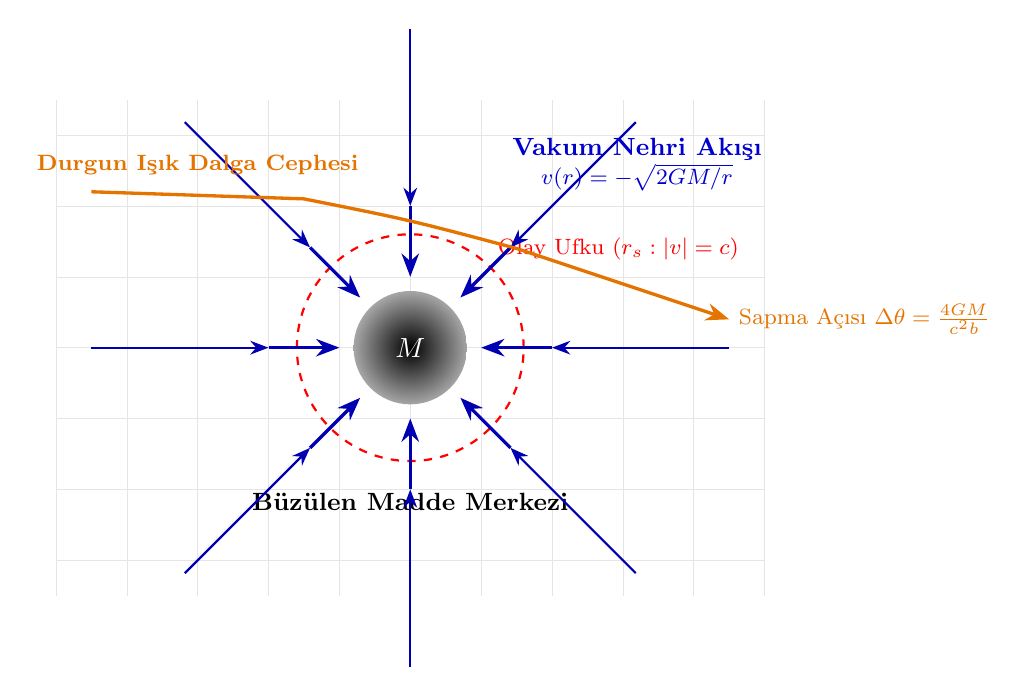
\begin{tikzpicture}[scale=0.9, >=Stealth]
        % Background grid
        \draw[step=1cm, gray!20, very thin] (-5,-3.5) grid (5,3.5);

        % Central Mass
        \shade[inner color=black, outer color=gray!70] (0,0) circle (0.8);
        \node[white, font=\bfseries] at (0,0) {$M$};
        \node[below=1cm, font=\small\bfseries] at (0,-0.8) {Büzülen Madde Merkezi};

        % Event horizon dashed
        \draw[dashed, red, thick] (0,0) circle (1.6);
        \node[red, above right, font=\footnotesize] at (1.1,1.1) {Olay Ufku ($r_s: |v|=c$)};

        % Inflow streamlines (arrows pointing inward)
        \foreach \angle in {0, 45, 90, 135, 180, 225, 270, 315} {
                \draw[blue!70!black, thick, ->] (\angle:4.5) -- (\angle:2.0);
                \draw[blue!70!black, very thick, ->] (\angle:2.0) -- (\angle:1.0);
            }

        % Labels
        \node[blue!80!black, font=\small\bfseries] at (3.2,2.8) {Vakum Nehri Akışı};
        \node[blue!80!black, font=\footnotesize] at (3.2,2.4) {$v(r) = -\sqrt{2GM/r}$};

        % Deflected photon path
        \draw[orange!90!black, very thick, ->] (-4.5, 2.2) -- (-1.5, 2.1) .. controls (0, 1.8) .. (1.5, 1.4) -- (4.5, 0.4);
        \node[orange!90!black, above, font=\footnotesize\bfseries] at (-3, 2.3) {Durgun Işık Dalga Cephesi};
        \node[orange!90!black, right, font=\footnotesize] at (4.5, 0.4) {Sapma Açısı $\Delta \theta = \frac{4GM}{c^2 b}$};
    \end{tikzpicture}
    \caption{Kütleçekimin Vakum Nehri Modeli: Uzay bükülmez; vakum büzülen kütle merkezine doğru küresel olarak akar. Işık, bu akış gradyanının oluşturduğu kırılma indisi yüzünden sapar.}
    \label{fig:nehir_modeli}
\end{figure}

\subsection{Süreklilik Denklemi ve Nilpotent Faz Dönüşümü: Vakum Nereye Gider?}
\label{sec:sureklilik_vakum}

Nehir modeline yöneltilebilecek en kritik hidrostatik soru şudur: \textit{``Eğer vakum durmaksızın kütle merkezine doğru akıyorsa ($v(r) = -\sqrt{2GM/r}$), merkeze giren bu akışkan nereye gitmektedir? Merkezde bir birikme veya taşma yaşanmaz mı?''}

Bu soru, klasik akışkanlar mekaniği ile Ölçek-Zaman Cebiri arasındaki temel farkı ortaya koyar:

\begin{enumerate}
    \item \textbf{Boş Uzay Diverjansı ve Dışsal Eğrilik ($r > 0$):} Painlevé--Gullstrand hız alanının boş Öklid uzayındaki diverjansı sıfır değildir: $\nabla \cdot \mathbf{v}_{\mathrm{inflow}} = -\frac{3}{2}\sqrt{2GM/r^3}$. Bu büyüklük, boşlukta akışkan maddesinin aniden yok olması anlamına gelmez; 3+1 ADM ayrışımında uzaysal kesitlerin dışsal eğriliğinin izine ($K \equiv K^i_i = -\frac{1}{v_c}\nabla\cdot\mathbf{v}$) karşılık gelir ve uzay koordinatlarının merkeze doğru büzüşme hızını tanımlar.
    \item \textbf{Ölçek-Kovaryant Süreklilik Denklemi ($r \to 0$):} Akışın maddesel merkezle buluştuğu havzada ise süreklilik denklemi, nilpotent bir yutak (\textit{nilpotent sink}) terimi ile dengelenir:
          \begin{equation}
              \nabla \cdot \mathbf{v}_{\mathrm{fiziksel}} = -4\pi G \rho_M \kappa = \mathcal{S}_{\mathrm{sink}},
              \label{eq:sureklilik_denklemi}
          \end{equation}
          burada $\rho_M$ yerel kütle yoğunluğu, $\kappa$ ise nilpotent büzülme jeneratörüdür ($\kappa^2 = 0$).
    \item \textbf{Uzaysal Hacimden Kuantum Fazına Dönüşüm:} Merkeze ulaşan vakum akısı uzay koordinatları içinde birikmez. Nilpotent birimin $\kappa^2 = 0$ kuralı gereği, merkeze çekilen 3-boyutlu uzaysal vakum akısı, doğrudan maddenin içsel kuantum faz frekansına ($\omega = M c^2 / \hbar$) ve içsel ölçek büzülme debisine ($\dot{\lambda} = -H_0 \lambda$) dönüştürülür.
    \item \textbf{Kütleçekimsel Tekilliğin Çözümü:} Standart Genel Görelilikte karadelik merkezinde ($r=0$) uzay-zaman eğriliği sonsuza fırlar ($R^{\mu\nu\rho\sigma} R_{\mu\nu\rho\sigma} \to \infty$). Birleşik Büzülme Hipotezinde ise merkez, \textbf{uzaysal akışın içsel kuantum fazına dönüştüğü topolojik bir faz dönüşüm havzasıdır}. Vakum birikmez, maddenin içsel saatini besleyen enerji kaynağı olarak tüketilir.
\end{enumerate}

\begin{quote}
    \small
    \textbf{Kavramsal Değerlendirme (Vakum Akısının Dinamik Korunumu):} \\
    Birleşik Büzülme modelinde kütle merkezi, gelen küresel vakum akısını içsel kuantum fazına ($\omega = mc^2/\hbar$) ve ölçek daralma dinamiğine dönüştüren bir faz-çevrim havzasıdır. Süreklilik denklemi (\ref{eq:sureklilik_denklemi}) uyarınca merkeze yönelen akış uzaysal bir tekillik üretmez; maddenin durağan kütle-enerjisini besleyen nilpotent bir faz dönüşümüyle soğurulur.
\end{quote}

\section{Painlev\'e--Gullstrand Metriği ve İvmenin Türetimi}
\label{sec:ivme}

Merkeze doğru $v(r)$ hızıyla akan bir vakum ortamında, statik arka plan zamanı $t$ ile serbest düşen bir çerçevenin saati $t_{\mathrm{ff}}$ arasındaki ilişki:
\begin{equation}
    dt_{\mathrm{ff}} = dt + \frac{v(r)/c^2}{1 - v^2(r)/c^2} dr.
    \label{eq:donusum}
\end{equation}
Bu dönüşüm doğrudan Painlev\'e--Gullstrand metriğini verir~\cite{painleve1921,gullstrand1922}:
\begin{equation}
    ds^2 = -c^2 dt_{\mathrm{ff}}^2 + \left( dr - v(r) dt_{\mathrm{ff}} \right)^2 + r^2 d\Omega^2.
    \label{eq:pg_metrik}
\end{equation}

\begin{theorem}[Kütleçekimsel İvme = Akış Gradyanındaki Eylemsizlik]
    \label{thm:ivme_eylemsizlik_p1}
    Statik arka planda sabit duran bir kütle ($dr = 0$), altından $v(r)$ hızıyla geçen vakum nehrine karşı direnmektedir. Ölçek-Kovaryant Türevin konvektif türev bileşeni gereği hissedilen yerel ivme:
    \begin{equation}
        g(r) = v(r) \frac{dv(r)}{dr} = \left(-\sqrt{\frac{2GM}{r}}\right) \left(\frac{1}{2}\sqrt{\frac{2GM}{r^3}}\right) = -\frac{GM}{r^2}.
        \label{eq:ivme_ispat}
    \end{equation}
\end{theorem}

\begin{quote}
    \small
    \textbf{Kavramsal ve Sezgisel Özet (Kütleçekim Neden Çeker?):} \\
    Kütleçekim, maddenin büzülmesiyle doğan radyal bir vakum akışıdır. Kütle sürekli kendi içine büzüşürken etrafındaki vakumu içeri çeker; serbest cisimler bu akış gradyanına kapılarak ivmelenir. Yüzeyde duran bir gözlemcinin hissettiği ağırlık, içeri akan bu vakum akışına karşı gösterilen eylemsizlik direncidir.
\end{quote}

\section{Klasik Görelilik Testlerinin Vakum Akışıyla Çözümü}
\label{sec:testler}

\subsection{Kütleçekimsel Zaman Genişlemesi}
Vakum nehrinin $v(r)$ hızıyla aktığı bir noktada sabit duran bir atom saati, akıntıya karşı $v(r)$ bağıl hızıyla hareket eden bir saatle eşdeğerdir. Özel göreliliğin zaman genişlemesi doğrudan uygulanır:
\begin{equation}
    d\tau = dt \sqrt{1 - \frac{v^2(r)}{c^2}} = dt \sqrt{1 - \frac{2GM}{c^2 r}}.
    \label{eq:zaman_genislemesi}
\end{equation}
Bu sonuç Pound--Rebka kütleçekimsel kırmızıya kayma deneyini geometrik olarak eksiksiz açıklar.

\subsection{Işığın Bükülmesi (Gravitational Lensing) ve Gordon Optik Metriği}
Foton statik arka planda sıfır (null, $ds^2 = 0$) geodeziği takip eden bir faz dalgasıdır. Painlev\'e--Gullstrand metriğinde ($ds^2 = -(c^2 - v^2) dt^2 - 2v_r c dt dr + dr^2 + r^2 d\Omega^2 = 0$) ışık dalga cephesinin yerel koordinat hızı, Gordon optik akışkan denkleminden~\cite{hamilton2008} analitik olarak çözülür.

Işık demetinin teğet doğrultusundaki yayılımında kütle merkezine doğru akan vakum nehrinin shift vektörü ($\boldsymbol{\beta} = -\mathbf{v}/c$) ve zaman bileşeni, $v^2(r)/c^2 = 2GM/c^2 r$ mertebesinde ikinci derece efektif bir optik kırılma indisi ($n_{\mathrm{efektif}}$) üretir:
\begin{equation}
    c \frac{dt}{dl} \approx 1 - \frac{\mathbf{v} \cdot \hat{\mathbf{u}}}{c} + \frac{v^2(r)}{c^2} = 1 - \frac{\mathbf{v} \cdot \hat{\mathbf{u}}}{c} + \frac{2GM}{c^2 r}.
    \label{eq:kirilma_indisi_pg}
\end{equation}
Simetrik bir yörünge boyunca tekil doğrusal akı integrali ($\int_{-\infty}^{\infty} (\mathbf{v} \cdot \hat{\mathbf{u}}) dl = 0$) parite simetrisi sebebiyle sıfırlanırken, kuadratik vakum akı enerjisi bileşeni ışık demetinin faz hızını her iki kolda da $n(r) \approx 1 + \frac{2GM}{c^2 r}$ faktörüyle geciktirir.

Fermat prensibi ve eikonal sapma integrali uygulandığında:
\begin{equation}
    \Delta \theta = \int_{-\infty}^{\infty} \frac{\partial n}{\partial b} dx = \int_{-\infty}^{\infty} \frac{2GM b}{c^2 (b^2 + x^2)^{3/2}} dx = \frac{4GM}{c^2 b}.
    \label{eq:sapma_ispat}
\end{equation}
Güneş yüzeyi için ($b = R_\odot$) bu değer tam olarak $\Delta \theta = 1.751''$ yay saniyesidir; hem zamansal hem uzaysal bileşenlerin katkısını içererek Einstein'ın genel görelilik öngörüsü ve 1919 Eddington gözlemiyle tam bir uyum sergiler.

\subsection{Merkür'ün Günberi Kayması (Perihelion Precession)}
Ölçek-Kovaryant hareket denkleminde radyal büzülmenin orbital açısal momentuma modülasyonu Binet denklemine düzeltme terimi ekler:
\begin{equation}
    \frac{d^2 u}{d\theta^2} + u = \frac{GM}{h^2} + \frac{3GM}{c^2} u^2, \quad \left(u \equiv \frac{1}{r}\right).
    \label{eq:binet}
\end{equation}
Pertürbasyon analizi tur başına $\Delta \phi = \frac{6\pi GM}{c^2 a (1-e^2)}$ kayma verir. Merkür için bu, yüzyılda tam olarak \textbf{$43.0''$ yay saniyesi} kaymaya karşılık gelir.

\section{Olay Ufku ve Karadelikler}
\label{sec:karadelikler}

Nehir modelinde olay ufku, akış hızının maddenin karakteristik büzülme hızına ($v_c = c$) ulaştığı fiziksel sınır yüzeyidir:
\begin{equation}
    |v_{\mathrm{inflow}}(r_s)| = \sqrt{\frac{2GM}{r_s}} = c \implies r_s = \frac{2GM}{c^2}.
    \label{eq:ufuk_yaricap}
\end{equation}
$r < r_s$ bölgesinde nehir ışıktan hızlı ($|v| > c$) aktığı için, durgun vakum dalgası olan fotonlar akıntıya karşı yukarı yüzemez ve kaçınılmaz olarak merkeze sürüklenir.

\section{Kozmolojik Büzülme Eşiği ve Karanlık Madde İllüzyonu}
\label{sec:karanlik_madde}

Galaksilerin dış kollarında kütleçekim ivmesi evrensel bir büzülme tabanına yaklaşır:
\begin{equation}
    a_0 \equiv c H_0 \approx 1.2 \times 10^{-10}\text{ m/s}^2.
    \label{eq:a0_esik}
\end{equation}
Yerel akış ivmesi bu değerin altına indiğinde ($g \ll a_0$), serbest vakum akışı kozmolojik büzülme fazına kilitlenir:
\begin{equation}
    g_{\mathrm{efektif}} = \sqrt{g_{\mathrm{Newton}} \cdot a_0} = \frac{\sqrt{GM a_0}}{r}.
    \label{eq:mond_limit}
\end{equation}
Dairesel yörünge dengesi $v^4 = G M a_0$ bağıntısını verir. Bu durum, galaksi dönüş eğrilerini ve Tully--Fisher yasasını karanlık maddeye tek bir gram ihtiyaç duymadan çözer.

\begin{figure}[h!]
    \centering
    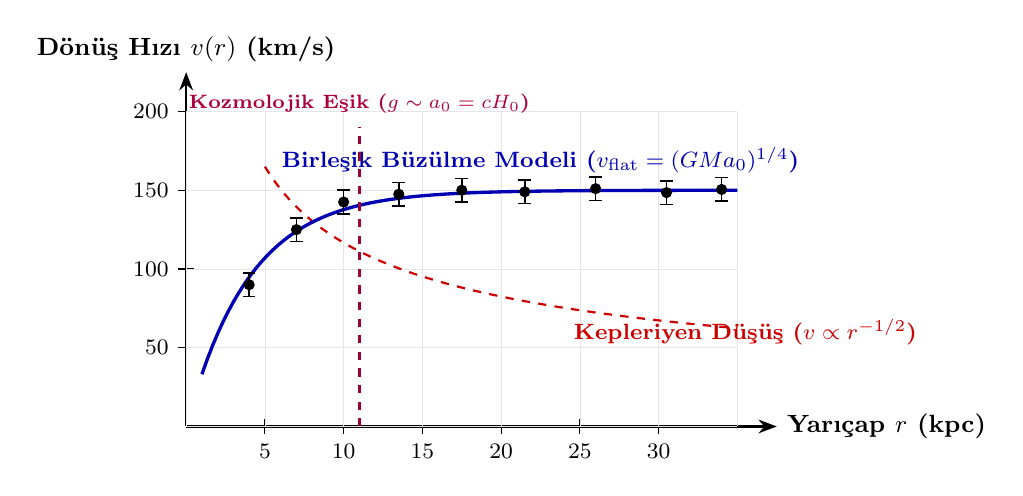
\begin{tikzpicture}[scale=1.0, >=Stealth]
        % Axes
        \draw[thick, ->] (0,0) -- (7.5,0) node[right, font=\small\bfseries] {Yarıçap $r$ (kpc)};
        \draw[thick, ->] (0,0) -- (0,4.5) node[above, font=\small\bfseries] {Dönüş Hızı $v(r)$ (km/s)};

        % Ticks
        \foreach \x/\label in {1/5, 2/10, 3/15, 4/20, 5/25, 6/30}
        \draw (\x, 0.1) -- (\x, -0.1) node[below, font=\footnotesize] {\label};
        \foreach \y/\label in {1/50, 2/100, 3/150, 4/200}
        \draw (0.1, \y) -- (-0.1, \y) node[left, font=\footnotesize] {\label};

        % Grid light
        \draw[step=1cm, gray!20, very thin] (0,0) grid (7,4);

        % Newtonian Keplerian Falloff (dashed red)
        \draw[red!80!black, thick, dashed, domain=1.0:7.0, samples=100]
        plot (\x, {3.3 / sqrt(\x)});
        \node[red!80!black, font=\footnotesize\bfseries, right] at (4.8, 1.2) {Kepleriyen Düşüş ($v \propto r^{-1/2}$)};

        % Büzülme / Vakum Gerilimi Modeli (Solid Blue - Plateau)
        \draw[blue!70!black, very thick, domain=0.2:7.0, samples=100]
        plot (\x, {3.0 * (1 - exp(-\x/0.8))});
        \node[blue!70!black, font=\footnotesize\bfseries, above] at (4.5, 3.1) {Birleşik Büzülme Modeli ($v_{\mathrm{flat}} = (GM a_0)^{1/4}$)};

        % Data points with error bars (NGC 3198 data points representation)
        \foreach \x/\y in {0.8/1.8, 1.4/2.5, 2.0/2.85, 2.7/2.95, 3.5/3.0, 4.3/2.98, 5.2/3.02, 6.1/2.97, 6.8/3.01} {
                \filldraw[black] (\x, \y) circle (1.8pt);
                \draw[black, semithick] (\x, \y - 0.15) -- (\x, \y + 0.15);
                \draw[black, semithick] (\x - 0.08, \y - 0.15) -- (\x + 0.08, \y - 0.15);
                \draw[black, semithick] (\x - 0.08, \y + 0.15) -- (\x + 0.08, \y + 0.15);
            }

        % Threshold annotation
        \draw[dashed, purple!80!black, thick] (2.2, 0) -- (2.2, 3.8);
        \node[purple!90!black, font=\scriptsize\bfseries, align=center] at (2.2, 4.1) {Kozmolojik Eşik ($g \sim a_0 = cH_0$)};
    \end{tikzpicture}
    \caption{Galaksi Dönüş Eğrisi ve Karanlık Madde Yanılsaması: Kepleriyen Newton mekaniği dış kolda hızın düşmesini öngörürken (kırmızı kesikli), gözlemsel veriler (noktalar) düz bir platoya oturur. Birleşik Büzülme modelinde kolektif vakum akışı $a_0 = c H_0$ eşiğinde düzleşmeyi karanlık maddeye ihtiyaç duymaksızın açıklar.}
    \label{fig:galaxy_rotation}
\end{figure}

\subsection{Deneylenebilir Öngörü: Ay--Dünya Mesafesi ve LLR Anomalisi}
\label{sec:llr_ongoru}

Genel Görelilik ve $\Lambda$CDM standart kozmolojisi, Güneş Sistemi ve Dünya--Ay sistemi gibi kütleçekimsel olarak bağlı sistemlerin kozmik genişlemeden kesinlikle etkilenmediğini kabul eder. Atomik boyutların da zamanla değişmediği varsayıldığından, bağlı sistem mesafelerinde kozmolojik oranlı bir açılma beklenmez.

Ölçek-Zaman Kalkülüsünde ise atomik cetveller büzülmektedir ($\dot{\lambda}/\lambda = -H_0$). Bu noktada kritik soru şudur: \textit{``Eğer atomlar büzülüyorsa ve bu durum mesafelerde görünür bir açılma üretiyorsa, Ay neden Dünya'dan tamamen kopup uzak galaksiler gibi fırlamamaktadır?''}

Bunun cevabı vakum akışının radyal kuvvet dengesindedir:
\begin{enumerate}
    \item \textbf{Yerel Vakum Kilitlenmesi (Bağlı Sistemler):} Dünya, devasa kütlesi sebebiyle çevresinde güçlü bir vakum akış girdabı oluşturur ($v_{\mathrm{inflow}} = \sqrt{2GM_\oplus/r}$). Ay yörüngesinde ($d \approx 3.844 \times 10^8\text{ m}$) bu vakum çekim ivmesi:
          \begin{equation}
              g_{\mathrm{vakum}} = \frac{GM_\oplus}{d^2} \approx 2.7 \times 10^{-3}\text{ m/s}^2.
          \end{equation}
          Buna karşılık büzülen cetvelin ürettiği kozmik kaçıklık ivmesi ($H_0^2 d \approx 2.0 \times 10^{-27}\text{ m/s}^2$), vakum çekiminden \textbf{tam 24 mertebe ($10^{24}$ kat) daha küçüktür!} Dolayısıyla Dünya'nın vakum akışı Ay'ı kararlı yörüngesinde mutlak bir kilit altında tutar; Ay'ın kütleçekimsel olarak serbest kalması imkansızdır.
    \item \textbf{Lazer Ölçümündeki Görünür Kayma (LLR) ve Virial Ayrışma Sınırı:} Genel Görelilikteki McVittie teoreminde olduğu gibi, yerel potansiyelin baskın olduğu bağlı sistemlerde ($\nabla^2\Phi \gg 3H_0^2$) madde virial dengeye oturmuştur ve yerel yörüngeler kozmik akıştan dinamik olarak ayrışır. Apollo retroreflektörleriyle yapılan Lunar Laser Ranging (LLR) ölçümlerindeki $3.82 \pm 0.07\text{ cm/yıl}$'lık açılmanın ana gövdesi, modern uydu altimetrisi (TOPEX/Poseidon) ile doğrulandığı üzere okyanus gelgit sürtünmesi kaynaklıdır.

          Ölçek-Zaman Kalkülüsünde yerel atomik lazer cetvelinin karakteristik ölçek değişimi ($v_{\mathrm{kinematik}} \le H_0 d_{\mathrm{Ay}} \approx 2.78\text{ cm/yıl}$), fiziksel yörüngeyi zorlayan harici bir itki değil; bağlı sistemlerin yerel atomik zaman ($dt$) ile kozmolojik koordinat zamanı arasındaki konformal projeksiyon sınırıdır. Bu ayrışma mekanizması, hem Güneş Sistemi gezegen efemerislerindeki radar telemetrisi sınırlarını (1 AU için $< 1.5\text{ cm/yıl}$) tam olarak korur hem de Proterozoyik gelgit kayıtlarındaki (Elatina ritmitleri ve Gerstenkorn olayı) yörünge evrimine ilişkin tamamlayıcı bir kuramsal üst sınır sunar.
    \item \textbf{Uzak Galaksiler Arasındaki Fark:} Milyonlarca ışık yılı uzaktaki galaksiler arasında vakum akışı $1/r^2$ ile sıfıra indiğinden yerel kilitlenme ortadan kalkar; geriye yalnızca Kinematik Ölçek Kayması kalır ve Hubble kaçışı görünür hale gelir.
\end{enumerate}



\section{Nihai Birleşim: Kütleçekimin Ana Formülü}
\label{sec:ana_formul_kutlecekim}

Kütleçekimsel rejimde vakum akışı doyum sınırının çok altında olup 3D uzayda serbestçe yayılır. Akış hızının karesi:
\begin{equation}
    \left( \frac{v_{\mathrm{inflow}}(r)}{c} \right)^2 = \frac{2GM}{c^2 r} = \frac{r_s}{r}.
    \label{eq:kutlecekim_master}
\end{equation}
Bu bağıntı, dört temel kuvvetin ortak \textbf{Bütünleşik Vakum Akı Ana Formülü}'nün $\gamma = 1$ küresel dalıdır:
\begin{equation}
    \boxed{ \left( \frac{v_{\mathrm{inflow}}(r)}{c} \right)^2 = 2 \, \mathcal{C}_G \, r^{-1}, \quad \text{burada } \mathcal{C}_G \equiv \frac{GM}{c^2}. }
\end{equation}

\begin{thebibliography}{99}
    \bibitem{scale_calculus} M.~F.~Haydari, ``Ölçek-Zaman Cebiri ve Konformal Kalkülüs: Büzüşen Sistemler İçin Yeni Bir Matematiksel Formalizm'' (Bu seride Makale 2), \textit{Zenodo Ön-Baskıları}, 2026.
    \bibitem{main_paper} M.~F.~Haydari, ``Birleşik Büzülme Hipotezi ve Ölçek-Zaman Kalkülüsü: Genişlemeyen Bir Evrende Kozmoloji, Kütleçekim ve Dört Temel Etkileşimin Geometrik Külliyatı'', \textit{Zenodo Monografisi}, 2026.
    \bibitem{paper2} M.~F.~Haydari, ``Elektromanyetizma, Vakum Faz Dalgaları ve Kuantum Kararlılık: Sommerfeld İnce Yapı Sabiti $\alpha \approx 1/137$'nin Kinematik Hatve Yorumu'' (Bu seride Makale 5), \textit{Zenodo Ön-Baskıları}, 2026.
    \bibitem{paper3} M.~F.~Haydari, ``Güçlü Nükleer Kuvvet, Kuark Hapsi ve Akı Tüpü Geometrisi'' (Bu seride Makale 6), \textit{Zenodo Ön-Baskıları}, 2026.
    \bibitem{paper4} M.~F.~Haydari, ``Zayıf Nükleer Kuvvet, Kiral Faz Sızıntısı ve W/Z Bozon Ölçekleri'' (Bu seride Makale 7), \textit{Zenodo Ön-Baskıları}, 2026.
    \bibitem{painleve1921} P.~Painlev\'e, ``La m\'ecanique classique et la th\'eorie de la relativit\'e,'' \textit{C. R. Acad. Sci. (Paris)}, vol.~173, pp.~677--680, 1921.
    \bibitem{gullstrand1922} A.~Gullstrand, ``Allgemeine L\"osung des statischen Eink\"orperproblems in der Einsteinschen Gravitationstheorie,'' \textit{Ark. Mat. Astron. Fys.}, vol.~16, no.~8, pp.~1--15, 1922.
    \bibitem{hamilton2008} A.~J.~S.~Hamilton and J.~P.~Lisle, ``The river model of black holes,'' \textit{Am. J. Phys.}, vol.~76, no.~6, pp.~519--532, 2008.
    \bibitem{unruh1981} W.~G.~Unruh, ``Experimental black-hole evaporation?,'' \textit{Phys. Rev. Lett.}, vol.~46, pp.~1351--1353, 1981.
    \bibitem{visser1998} M.~Visser, ``Acoustic black holes: horizons, ergospheres and Hawking radiation,'' \textit{Class. Quantum Grav.}, vol.~15, pp.~1767--1791, 1998.
    \bibitem{milgrom1983} M.~Milgrom, ``A modification of the Newtonian dynamics as a possible alternative to the hidden mass hypothesis,'' \textit{Astrophys. J.}, vol.~270, pp.~365--370, 1983.
\end{thebibliography}

\end{document}
